\section{Auswertung}
\label{sec:Auswertung}

\subsection{Brechungsindex über die Fresnel Formel bestimmen}
Der gemessene Dunkelstrom ist $I_\text{dunkel} = 1.4 \unit{\nano\ampere}$. Dieser wird bei den folgenden Berechnungen von den gemmesenen Intensität abgezogen.
Die gemessenen Intesitäten für das senkrecht polarisiertem Licht sind in der Tabelle \ref{tab:senk} und 
die für parallel polarisiertem Licht in Tabelle \ref{tab:para} dargestellt.
Zur Berchnung des Brechungsindex für Silizium werden die Formeln \ref{eq:Esenk} und \ref{eq:Epara} verwendet.
Dabei gilt 
\begin{equation*}
  \frac{E_r}{E_e} = \sqrt{\frac{I(\alpha)}{I_0}} = E,
\end{equation*}
da die Intesität des Lichts proportional zum Quadrat der Amplitude des E-Feldes.
Bei beiden Messungen wurde ein Nullstrom von $I_0 = 180 \unit{\micro\ampere}$ gemessen.
Die Formeln \ref{eq:Esenk} und \ref{eq:Epara} werden nach $n$ umsgestellt.
Damit ergibt sich für den Brechungsindex bei senkrecht polarisiertem Licht
\begin{equation}
  n_\parallel = \Bigl(\frac{E+1}{E-1}\Bigr)^2\frac{1}{2 \cos(\alpha)^2}+\sqrt{\frac{1}{4 \cos(\alpha)^2}\Bigl(\frac{E+1}{E-1}\Bigr)^4-\Bigl(\frac{E+1}{E-1}\Bigr)^2 \tan(\alpha)^2}
\end{equation}
und für den Brechungsindex bei senkrecht polarisiertem Licht
\begin{equation}
  n_\perp = \sqrt{\frac{1+ E^2+ 2 E \cos(2 \alpha)}{1- 2 E+ E^2}}.
\end{equation}
Die Ergebnisse der Brechungindexe werden ebenfalls in der Tabelle \ref{tab:senk} und \ref{tab:para} dargestellt.
\begin{table}[H]
  \centering
  \caption{Gemessene Intensitäten und berechneter Brechungsindex bei senkrecht plarisierten Licht.}
  \label{tab:senk}
  \begin{tabular}{c c c c c c}
    \toprule
    $\alpha /°$ & $I / \unit{\micro\ampere}$ & $n$ & $\alpha /°$ & $I / \unit{\micro\ampere}$ & $n_\perp$\\
    \midrule          
    4  &  54  & 3.41    & 48 &  92   & 4.09   \\
    6  &  60  & 3.71    & 50 &  92   & 3.94   \\ 
    8  &  64  & 3.91    & 52 &  97   & 4.09    \\
    10 &  66  & 4.01    & 54 &  96   & 3.85    \\
    12 &  64  & 3.87    & 56 &  100  & 3.92    \\
    14 &  62  & 3.73    & 58 &  100  & 3.72    \\
    16 &  66  & 3.92    & 60 &  100  & 3.53    \\
    18 &  64  & 3.77    & 62 &  100  & 3.33   \\ 
    20 &  70  & 4.06    & 64 &  100  & 3.13    \\
    22 &  70  & 4.01    & 66 &  110  & 3.44    \\
    24 &  72  & 4.07    & 68 &  110  & 3.19    \\
    26 &  72  & 4.01    & 70 &  115  & 3.20    \\
    28 &  72  & 3.94    & 72 &  120  & 3.20    \\
    30 &  74  & 3.99    & 74 &  130  & 3.52    \\
    32 &  76  & 4.02    & 76 &  135  & 3.50   \\ 
    34 &  78  & 4.06    & 78 &  140  & 3.45   \\
    36 &  78  & 3.96    & 80 &  144  & 3.26   \\
    38 &  82  & 4.10    & 80 &  144  & 2.92   \\
    40 &  84  & 4.11    & 82 &  147  & 1.94   \\
    42 &  86  & 4.12    & 84 &  140  & 1.04   \\
    44 &  88  & 4.12    & 86 &  70   & (4.88) \\ 
    46 &  90  & 4.11    &    &       &        \\                 
    \bottomrule
  \end{tabular}
\end{table}
      
\begin{table}[H]
  \centering
  \caption{Gemessene Intensitäten und berechneter Brechungsindex bei parallel plarisierten Licht.}
  \label{tab:para}
  \begin{tabular}{c c c c c c}
    \toprule
    $\alpha /°$ & $I / \unit{\micro\ampere}$ & $n$ & $\alpha /°$ & $I / \unit{\micro\ampere}$ & $n_\parallel$\\
    \midrule 
    6  &  50  & 3.24     & 48 &  28   &  3.35  \\ 
    8  &  50  & 3.25     & 50 &  27   &  3.43   \\
    10 &  50  & 3.27     & 52 &  24   &  3.39   \\
    12 &  49  & 3.24     & 54 &  20   &  3.29   \\
    14 &  48  & 3.22     & 56 &  20   &  3.47   \\
    16 &  48  & 3.25     & 58 &  18   &  3.52   \\
    18 &  42  & 3.00     & 60 &  14   &  3.43  \\
    20 &  47  & 3.27     & 62 &  14   &  3.66   \\
    22 &  46  & 3.26     & 64 &  12   &  3.75   \\
    24 &  45  & 3.25     & 66 &  11   &  3.96   \\
    26 &  44  & 3.25     & 68 &  9.6  &  4.16   \\
    28 &  44  & 3.31     & 70 &  8    &  4.38   \\
    30 &  41  & 3.22     & 72 &  8.2  &  4.89   \\
    32 &  41  & 3.28     & 74 &  8.6  &  5.57   \\
    34 &  37  & 3.15     & 76 &  9.6  &  6.54   \\
    36 &  38  & 3.28     & 78 &  10   &  7.71   \\
    38 &  37  & 3.31     & 80 &  12   &  9.71   \\
    40 &  36  & 3.35     & 82 &  21   &  14.60  \\
    42 &  34  & 3.34     & 84 &  30   &  22.74   \\
    44 &  32  & 3.34     & 86 &  50   &  46.27   \\
    46 &  30  & 3.34     &    &       &           \\
    \bottomrule
  \end{tabular}
\end{table}

\noindent Die berechneten Brechungsindexe werden nun gemittelt.
Damit ergibt sich 
\begin{equation*}
  \overline{n_\perp} = 3.65 \pm
\end{equation*}
und\begin{equation*}
  \overline{n_\parallel} = 5.62 \pm
\end{equation*}    

\subsection{Brewsterwinkel}
    








\begin{figure}
  \centering
  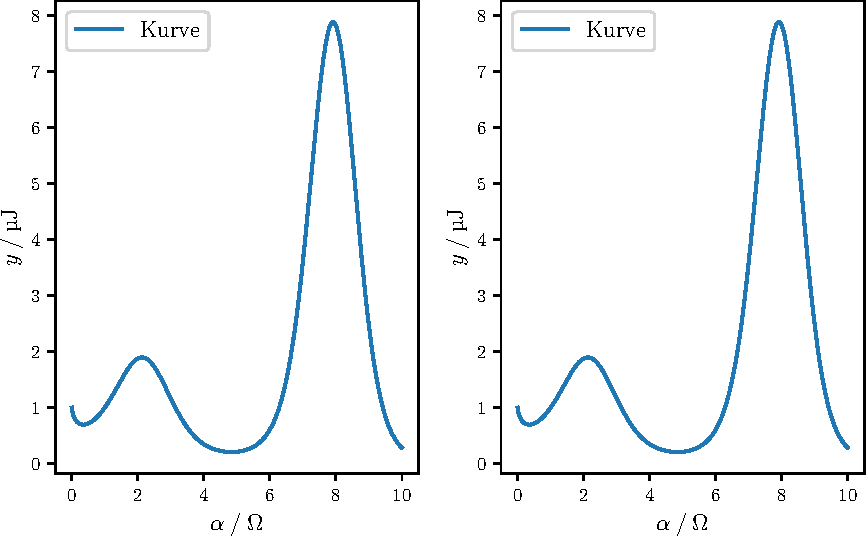
\includegraphics{plot.pdf}
  \caption{Plot.}
  \label{fig:plot}
\end{figure}


Siehe \autoref{fig:plot}!
